\subsection{Протокол Нидхема~---~Шрёдера}\index{протокол!Нидхема~---~Шрёдера|(}\label{section-protocols-needham-schroeder}
\selectlanguage{russian}

Протокол Нидхема~---~Шрёдера (\langen{Roger Needham, Michael Shroeder}, 1979,~\cite{Needham:Schroeder:1978}) похож на модифицированный протокол Wide-Mouth Frog, но отличается тем, что доверенный центр (Трент) во время работы основной части протокола не общается со вторым абонентом. Первый абонент получает от доверенного центра специальный пакет, который он без всякой модификации отправляет второму абоненту.

\begin{figure}[!htb]
    \centering
    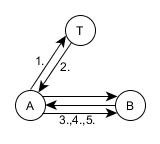
\includegraphics[width=0.5\textwidth]{pic/key_distribution-needham-schroeder}
    \caption{Схема взаимодействия абонентов и доверенного центра в протоколе Нидхема~---~Шрёдера\label{fig:key_distribution-needham-schroeder}}
\end{figure}

\begin{enumerate}
	\item $ Alice	\rightarrow \{ A, B, R_A \}						\rightarrow Trent $
	\item $ Trent	\rightarrow \{ E_A \left( R_A, B, K, E_B \left( K, A \right) \right) \}	\rightarrow Alice $
	\item $ Alice	\rightarrow \{ E_B \left( K, A \right) \}				\rightarrow Bob $
	\item $ Bob	\rightarrow \{ E_K \left( R_B \right) \}				\rightarrow Alice $
	\item $ Alice	\rightarrow \{ E_K \left( R_B - 1 \right) \}				\rightarrow Bob $
\end{enumerate}

Протокол обеспечивает и двустороннюю аутентификацию сторон, и, казалось бы, защиту от атак с повторной передачей (\langen{replay attack}). Последнее делается с помощью введения уже известных по модифицированному протоколу Wide-Mouth Frog случайных меток $R_A$ и $R_B$. Действительно, без знания ключа злоумышленник не сможет выдать себя за Алису перед Бобом (так как не сможет расшифровать пакет с зашифрованной меткой $R_B$). Однако, как мы договорились ранее во введении к этой главе, сам сессионный ключ не может считаться надёжным длительное время. Если злоумышленник сумеет в какой-то момент времени получить ранее использованный сессионный ключ $K$, он сможет убедить Боба, что он является Алисой, и что это новый сессионный ключ. Для этого ему понадобится переданный ранее по открытому каналу пакет из пункта 3 протокола.

\begin{enumerate}
	\item $ Eva		\rightarrow \{ A, B, R_A \}						\rightarrow Trent $
	\item $ Trent		\rightarrow \{ E_A \left( R_A, B, K, E_B \left( K, A \right) \right) \}	\rightarrow Alice $
	\item $ Alice		\rightarrow \{ E_B \left( K, A \right) \}				\rightarrow Bob $
	\item $ Bob		\rightarrow \{ E_K \left( R_B \right) \}				\rightarrow Alice $
	\item $ Alice		\rightarrow \{ E_K \left( R_B - 1 \right) \}				\rightarrow Bob $

		$\dots$ по прошествии некоторого времени $\dots$\\
	\item $ Eva~(Alice)	\rightarrow \{ E_B \left( K, A \right) \}				\rightarrow Bob $
	\item $ Bob		\rightarrow \{ E_K \left( R_B \right) \}				\rightarrow Eva~(Alice) $
	\item $ Eva (Alice)	\rightarrow \{ E_K \left( R_B - 1 \right) \}				\rightarrow Bob $
\end{enumerate}

Относительно мелкий недостаток протокола состоит ещё и в том, что во втором пакете доверенный центр в зашифрованном виде передаёт то, что в третьем шаге пересылается по открытому каналу ($E_B \left( K, A \right)$).

Если в протокол добавить метки времени, тем самым ограничив время возможного использования сессионного ключа, а также исправить мелкий недостаток с двойным шифрованием, можно получить протокол, который лежит в основе распространённого средства аутентификации <<Kerberos>> для локальных сетей.

\index{протокол!Нидхема~---~Шрёдера|)}
